\documentclass{article}

\usepackage[letterpaper, top=2cm, bottom=1.8cm, inner=1.8cm,
outer=1.8cm, foot=.25in]{geometry}

\setcounter{tocdepth}{1}

\usepackage{amsmath, amssymb}
\usepackage{comment}
\usepackage{graphicx}
%\usepackage[T1]{fontenc}
%\usepackage{ae, aecompl}
\usepackage[numbers]{natbib}

%%%%%%%%%%%%%%%%%%%%%%%%%%%%%%%%%%%%%%%%%%%%%%%%%%%%%%%%%%%%%%%%%%%%%%%%
%% math

%
% General
%

\DeclareMathOperator{\argmin}{arg\,min}
\DeclareMathOperator{\argmax}{arg\,max}

%
% Sets
%

\newcommand{\card} [1]{{\lvert #1 \rvert}}
\newcommand{\range}[1]{{\left\{ 1, \dots, #1 \right\}}}

%
% Linear algebra
%

\newcommand{\mat}  [1]{{\bf #1}}
\newcommand{\norm} [1]{{\lVert #1 \rVert}}
\newcommand{\vect} [1]{{\mbox{\boldmath $#1$}}}

%
% Probability. The CTAN `proba` package doesn't seem to be that good.
% TODO ensuremath does not seem to be a good idea.
%

\newcommand{\E}    [2]{{\textrm{E} \left[ #1 \mid #2 \right]}}
\newcommand{\LL}   [2]{{\ensuremath{ L \left( #1 \,\middle|\, #2 \right) }}}
\newcommand{\LLL}  [2]{{\ensuremath{ l \left( #1 \,\middle|\, #2 \right) }}}
\newcommand{\N}    [1]{{\ensuremath{ \# \left( \textrm{ #1 } \right) }}}
\newcommand{\PO}   [1]{{\Pr \left( #1 \right)}}
\newcommand{\PP}   [2]{{\PO{ #1 \,\middle|\, #2 }}}

%%%%%%%%%%%%%%%%%%%%%%%%%%%%%%%%%%%%%%%%%%%%%%%%%%%%%%%%%%%%%%%%%%%%%%%%
%% Theoretical computer science

%
% Computational complexity
%

\DeclareMathOperator{\bigO}{O}
\providecommand{\OO}[1]{\bigO\bigl(#1\bigr)}

%%%%%%%%%%%%%%%%%%%%%%%%%%%%%%%%%%%%%%%%%%%%%%%%%%%%%%%%%%%%%%%%%%%%%%%%
%% General text

% \emph toggles italics; \textit sets italics; \em is deprecated
\newcommand{\term} [1]{{\emph{#1\/}}} 

% We don't need to do append a ~ or \ because TeX already handles .,
% correctly. TODO figure out if italics are correct here
\newcommand{\foreign}[1]{{\textit{#1}}}
\newcommand{\ea}      {{\foreign{et~al.}}}
\newcommand{\eg}      {{\foreign{e.g.}}}
\newcommand{\ie}      {{\foreign{i.e.}}}
\newcommand{\TODO} [1]{{\textbf{TODO}: \textit{#1}}}

%%%%%%%%%%%%%%%%%%%%%%%%%%%%%%%%%%%%%%%%%%%%%%%%%%%%%%%%%%%%%%%%%%%%%%%%
%% Remarks. Collected from the pervasive but untraceable `remarks.tex`.

\newif\ifremark
\long\def\remark#1{
\ifremark%
    \begingroup%
    \dimen0=\columnwidth
    \advance\dimen0 by -0.25in%
    \setbox0=\hbox{\parbox[b]{\dimen0}{\protect\em\textcolor{red}{#1}}}
    \dimen1=\ht0\advance\dimen1 by 2pt%
    \dimen2=\dp0\advance\dimen2 by 2pt%
    \vskip 0.25pt%
    \hbox to \columnwidth{%
        \vrule height\dimen1 width 3pt depth\dimen2%
        \hss\copy0\hss%
        \vrule height\dimen1 width 3pt depth\dimen2%
    }%
    \endgroup%
\fi}

\newcommand{\remarkname}[2] {
    \remark{{\bf #1}:#2}
}


\def\LaTeXe{c}

\title{Collaborative Filtering for the NetFlix Challenge}
\author{Masahiro Ono and Yang Zhang}

\begin{document}

\maketitle

\tableofcontents

\section{Introduction}
\subsection{Project Overview}
We implemented and evaluated two approaches to collaborative filtering; mixture model and low-rank approximation. They are tested on a subset of the NetFlix Prize dataset. This report includes theoretical basis of each approaches and empirical results as well as the complexity analysis and the discussion about the feasibility for large scale problem.

\subsection{Dataset}


The NetFlix dataset is large: it contains 480,189 users, 17,770
movies, and 100,480,507 ratings. This scale of the problem is beyond the scope of the class project, and MATLAB's in-memory data management is also not amenable to datasets of such scale. Hence, we used much smaller data set with 51 movies and 892 users, which is a subset of the full Netflix Prize dataset. Those 51 movies and 892 users are chosen so that the resulting rating matrix is fully packed. We then divide the rating matrix into training and test data. Since we have the fully packed rating matrix, we can arbitrary arrange the \textit{sparsity ratio}\footnote{\textit{Sparsity ratio means the ratio of missing element in the rating matrix. The original Netflix Prize data has 99\% sparsity ratio.}} of the training data to evaluate the dependency of the performance on the sparsity ratio.  

In the following context we denote by $\mat{R}$ the rating matrix whose rows correspond to users
and columns correspond to movies, such that entry $r_{i,j} \in \range{5}$ is the rating given by user $i$ to movie $j$. We also denote by $n_U$ and $n_M$ the number of users and movies.  

\subsection{Performance Measure}
The performance of each algorithm is measured by root-mean-squre error (RMSE), which is defined as follows;
\begin{equation}
RMSE = \left[ \sum_{(i,j) \in I_T} ({\hat r}_{i,j} - r_{i,j})^2 \right]^\frac{1}{2}
\end{equation}
where $I_T$ is the set of indices of the ratings included in the test data and ${\hat r}_{i,j}$ is the estimated rating of $i$th user for $j$th movie. 


\section{Mixture Model}

We use a mixture model to cluster together ratings based on user types
and movie types. There are various other mixture models for
collaborative filtering; this model is the one presented in 6.867
lecture 15 and is known as the \term{flexible mixture
  model}~\cite{si03flexible}. A survey of various alternative models
can be found in~\cite{cmu-study}.

For this part of our project, we rigorously derived the E-M algorithm,
implement the algorithm in MATLAB, and analyzed its results. In the
following sections, we describe and justify the model, then derive the
E-M algorithm and analyze its complexity. Next, we describe our
implementation, and finally we evaluate its performance by using
\TODO{what should our performance metric be?}

\subsection{Overview}

We say that \term{each user} has a distribution over user types (\eg,
mostly romantic, a bit of an intellectual), and each movie has a
distribution over movie types (mostly horror, some action). Each pair
of user type and movie type has a distribution over ratings (\eg,
romantics tend to give horrors low ratings). The likelihood of
our model given the parameters is then
\begin{align}
  \LL{D}{\theta}
  =& \PP{ R_{1,1} = r_{1,1}, \dots, R_{n_U,n_M} = r_{n_U,n_M} }{
    \theta } \\
  =& \prod_{i,j} \sum_{u,m} \left[
    \PP{ R_{i,j} = r_{i,j} }{ U_{i,j} = u, M_{i,j} = m,
      \theta^R_{u,m} } \cdot 
    \PP{ U_{i,j} = u }{ \theta^U_i } \cdot
    \PP{ M_{i,j} = m }{ \theta^M_j }
  \right] \\
  =& \prod_{i,j} \sum_{u,m}
  \theta^R_{u,m}(r) \cdot \theta^U_i(u) \cdot \theta^M_j(m)
\end{align}
We see that there are three sets of parameters, and our approach is to
use an E-M algorithm to perform maximum likelihood estimation of these
parameters.

Each cell has its own user and movie type. What does all this mean?
Intuitively, we can think of each cell as the result of an \term{act}
of rating. Hence, every time a user rates a movie, we are randomly
sampling from among the user's multiple personalities (\eg, the
romantic in the user was rating this movie). We are also sampling from
among the movie's multiple aspects (the user saw this movie as a
horror movie). We will loosely use the term ``rating'' to mean either
the act of the rating or the rating value itself; hopefully the
meaning remains clear from the context.

It is natural to use multinomial distributions for generating the user
types for a user, and the movie types for a movie. We are also using
multinomial distributions to generate ratings given a user type and
movie type; this we do for simplicity. \TODO{have a better
  explanation?}

\TODO{insert figure here}
Figure (TODO) shows our graphical model.

\TODO{verify the following} Note that this model works for
collaborative filtering for a static set of users and movies (filling
in holes). New users/movies (augmenting our matrix with rows/columns
that contain no data) would indeed be difficult to provide
recommendations for regardless of model. However, even if these new
rows/columns had data available, our approach requires re-training the
model, because each user and each movie has its own distribution over
user types and movie types. \TODO{say something about how we can get a
  prior over these?}

\subsection{E-M Algorithm}

\subsubsection{M-step with complete data}

To derive the E-M algorithm, it is helpful to start by assuming that
we have ``complete data''---that is, for each of the (observed)
ratings $i,j$, we know precisely which user type $u$ and movie type
$m$ the rating belongs to. With this information, we can directly and
analytically find the parameters that maximize the likelihood of the
data. We can equivalently optimize the log-likelihood: $\arg
\max_\theta \LL{D}{\theta} = \arg \max_\theta \log \LL{D}{\theta}$.
\begin{align}
  \LLL{D}{\theta} =& \log \LL{D}{\theta} \\
  =& \sum_{i,j \in I} \left[
    \begin{aligned}
      & \log \PP{R_{i,j} = r_{i,j}}{U_{i,j} = u_{i,J}, M_{i,j} = m_{i,j},
        \theta^R} + \\
      & \log \PP{U_{i,j} = u_{i,j}}{\theta^U_i} +  \log \PP{M_{i,j} = m_{i,j}}{\theta^M_j}
    \end{aligned}
  \right] \\
  =& \sum_{i,j \in I} \left[
    \log \theta^R_{u_{i,j},m_{i,j}}(r_{i,j}) +
    \log \theta^U_i(u_{i,j}) +
    \log \theta^M_j(m_{i,j})
  \right] \\
  =& \sum_{r,u,m,i,j} n_{r,u,m,i,j} \left[
    \log \theta^R_{u,m}(r) + \log \theta^U_i(u) + \log \theta^M_j(m)
  \right]
\end{align}
Above, $n_{r,u,m,i,j}$ is 1 if rating $i,j$ has rating value $r$, user
type $u$, and movie type $m$, and 0 otherwise.

Implicit throughout the previous equations were a number of
constraints due to the fact that we're dealing with probabilities. In
particular,
\begin{align}
\sum_r \theta_{u,m}(r) =& 1 &
\sum_u \theta_i(u) =& 1 &
\sum_m \theta_j(m) =& 1
\end{align}
To allow ourselves to optimize the equations analytically, we can
incorporate these into the equation by using LaGrange multipliers
($\lambda$s below):
\begin{multline}
  \sum_{r,u,m,i,j} n_{r,u,m,i,j} \left[
    \log \theta^R_{u,m}(r) + \log \theta^U_i(u) + \log \theta^M_j(m)
  \right] + \\
  \left\{
    \lambda^R_{u,m} \left( 1 - \sum_r \theta^R_{u,m}(r) \right)
    \forall u,m 
  \right\} +
  \left\{
    \lambda^U_i \left( 1 - \sum_u \theta^U_i(u) \right)
    \forall i 
  \right\} +
  \left\{
    \lambda^M_j \left( 1 - \sum_m \theta^M_j(m) \right)
    \forall j
  \right\}
\end{multline}

To find the maximizing value of a parameter, we find the zeros of the
partial derivative with respect to that parameter. This turns out to
be straightforward for the above expression, because the parameters
are in separate terms, so that many terms in the sums and quantifiers
``disappear.''

For all $u,i$,
\begin{align}
  0 =& \frac{ \partial \LLL{D}{\theta} }{ \partial \theta^U_i(u) }
  = \sum_{r,m,j} \frac{ n_{r,u,m,i,j} }{ \theta^U_i(u) } - \lambda^U_i
  & \Rightarrow &&
  \theta^U_i(u) =& \frac{ \sum_{r,m,j} n_{r,u,m,i,j} }{ \lambda^U_i } \\
  1 =& \sum_u \theta^U_i(u) 
  = \sum_u \frac{ \sum_{r,m,j} n_{r,u,m,i,j} }{ \lambda^U_i }
  & \Rightarrow &&
  \lambda^U_i =& \sum_{r,u,m,j} n_{r,u,m,i,j} \\
  &&&& \therefore \theta^U_i(u) 
  =& \frac{ \sum_{r,m,j} n_{r,u,m,i,j} }{ \sum_{r,u,m,j} n_{r,u,m,i,j} }
  = \frac{ n_{u,i} }{ n_M } \label{eq:pui}
\end{align}
This makes intuitive sense, since $\theta^U_i(u) = \PP{U_{i,j} =
u}{\theta^U_i}$ for any movie $j$. The probability that we see the
romantic in a user is the number of her other ratings where it was the
romantic in her speaking, over her total number of ratings.

Similarly (almost symmetrically), we find:
\begin{align}
\forall m,j,\ \theta^M_j(m) =& \frac{ n_{m,j} }{ n_U }
&
\forall r,u,m,\ \theta^M_j(m) =& \frac{ n_{r,u,m} }{ n_{u,m} }
\label{eq:prum}
\end{align}

However, we do not have complete data---we do not have the above
counts, since we do not know the user-/movie-type assignments. Since
the incomplete data does not yield an analytical solution, we must use
a numerical approach, namely an E-M algorithm. This algorithm
iteratively updates the parameters in the M-step based on
intermediately calculated posteriors in the E-step. Essentially, we
use the posteriors to find the \term{expected} counts in the above
equations.

\subsubsection{E-step}

For all $i \in \range{n_M}, j \in \range{n_M}$, we calculate the
posterior.
\begin{align}
& \PP{ U_{i,j} = u, M_{i,j} = m }{ R = \mat{R}, \theta } \\
=& \PP{ U_{i,j} = u, M_{i,j} = m }{ R_{i,j} = r_{i,j}, \theta^U_i,
  \theta^M_j, \theta^R }
&&
\text{independencies can be seen in graphical model} \\
=& \frac{1}{Z} \left(
\begin{aligned}
& \PP{R_{i,j} = r_{i,j} }{U_{i,j} = u, M_{i,j} = m, \theta^R} \\
& \PP{U_{i,j} = u, M_{i,j} = m}{\theta^U_i, \theta^M_j}
\end{aligned} \right)
&& \text{by Bayes' rule; $Z$ is a normalizer} \\
=& \frac{1}{Z} \left(
\begin{aligned}
& \PP{R_{i,j} = r_{i,j} }{U_{i,j} = u, M_{i,j} = m, \theta^R} \\
& \PP{U_{i,j} = u }{\theta^U_i}
  \PP{M_{i,j} = m }{\theta^M_j}
\end{aligned} \right)
&& \text{independencies in graphical model} \\
=& \frac{1}{Z} \theta^R_{u,m}(r_{i,j}) \theta^U_i(u) \theta^M_j(m)
\label{eq:pumrij}
\end{align}
Above,
\begin{align}
  Z = \PP{R_{i,j} = r_{i,j}}{\theta} = \sum_{u,m} \PP{U = u, M = m}{R = r, \theta^U_i, \theta^M_j,
    \theta^R}
\end{align}
The above independencies can be verified from the moralized ancestral
graphs of our model, but de do not have space to illustrate these
graphs here.

For any $i,j$,
letting $U = U_{i,j}, M = M_{i,j}, R = R_{i,j}$,
we can marginalize the above joint distribution over $M$ and $U$
to get the distributions over $U$ and $M$, respectively:
\begin{align}
  \PP{U = u}{R = r, \theta^U_i, \theta^M_j, \theta^R}
  =& \sum_m \PP{U = u, M = m}{R = r, \theta^U_i, \theta^M_j, \theta^R}
\\
  \PP{U = u}{R = r, \theta^U_i, \theta^M_j, \theta^R}
  =& \sum_m \PP{U = u, M = m}{R = r, \theta^U_i, \theta^M_j, \theta^R}
\end{align}

\subsubsection{M-step}

Now we can use these posterior values to find expected counts in order
to update the parameters.

For all $i \in \range{n_U}$, for any $j \in \range{n_M}$,
\begin{align}
  \E{n_{u,i}}{\mat{R}, \theta}
  =& \E{ \sum_{r,m,j} n_{r,u,m,i,j} }{R = \mat{R}, \theta} \\
  =& \sum_{r,m,j} \E{ n_{r,u,m,i,j} }{R = \mat{R}, \theta} \\
  =& \sum_{r,m,j} \left[
    0 + 1 \cdot \PP{ R_{i,j} = r, U_{i,j} = u, M_{i,j} = m }{R = \mat{R}, \theta}
  \right] \\
  =& \sum_j \PP{U_{i,j} = u}{R = \mat{R}, \theta}
  && \text{marginalized $M$, observed $R$} \\
  =& \sum_j \PP{U_{i,j} = u}{R_{i,j} = r_{i,j}, \theta^R_{u,m},
    \theta^U_i, \theta^M_j}
  && \text{independencies in graph} \\
  {\theta^U_i}'(u)
  =& \E{ \frac{ n_{u,i}}{ n_M } }{\theta} && \text{by Eq. \ref{eq:pui}} \\
  =& \frac{1}{n_M} \sum_j \PP{U_{i,j} = u}{ R_{i,j} = r_{i,j}, \theta^R_{u,m},
    \theta^U_i, \theta^M_j }
  && \text{weighted sum over the row}
\end{align}

Similarly, for all $j \in \range{n_M}$,
\begin{align}
  {\theta^M_j}'(m) =&
  \frac{1}{n_U} \sum_i \PP{M = m}{
    R_{i,j} = r_{i,j}, \theta^R_{u,m}, \theta^U_i, \theta^M_j}
\end{align}

Finally, for all $u \in \range{k_U}, m \in \range{k_M}$,
\begin{align}
  {\theta^R_{u,m}}'(r)
  =& \E{ \frac{n_{r,u,m}}{n_{u,m}} }{\theta}
  = \frac{ \E{n_{r,u,m} }{\theta} }{ \E{n_{u,m}}{\theta} }
   \text{\TODO{how to justify this?}} \\
  =& \frac{\sum_{i,j: r_{i,j} = r} \PP{U_{i,j} = u, M_{i,j} = m}{
      R_{i,j} = r_{i,j}, \theta^R_{u,m}, \theta^U_i, \theta^M_j}
  }{ \sum_{i,j} \PP{U_{i,j} = u, M_{i,j} = m}{
      R_{i,j} = r_{i,j}, \theta^R_{u,m}, \theta^U_i, \theta^M_j} } \\
\end{align}

\subsection{Complexity Analysis}

Here is a break-down of various dimensions of our model and
algorithm. Each parameter involves ``weighted sums'' over some number
of components of the joint posterior over $U,M$ given the data $R$;
the third column is the number of terms (the cost of the
summations). The fourth column is the total complexity, the product of
the second and third columns.
\begin{center}
  \begin{tabular}{c|c|c|c}
    component & no.~parameters &
    no.~posterior components & complexity
    \\ \hline
    $\theta_R$ & $(k_R - 1) \cdot k_U \cdot k_M$ &
    $\OO{n_U \cdot n_M}$ &
    $\OO{k_R \cdot k_U \cdot k_M \cdot n_U \cdot n_M}$ \\
    $\theta_U$ & $(k_U - 1) \cdot n_U$ &
    $\OO{k_M \cdot n_M}$ & $\OO{k_U \cdot n_U \cdot k_M \cdot n_M}$ \\
    $\theta_M$ & $(k_M - 1) \cdot n_M$ &
    $\OO{k_U \cdot n_U}$ & $\OO{k_M \cdot n_M \cdot k_U \cdot n_U}$ \\
  \end{tabular}
\end{center}
(A multinomial of $k$ possible outcomes needs only $k-1$ parameters.)

The posterior joint distribution over $U,M$ given the data $R$ is in
Eq. \ref{eq:pumrij}. This table is of size $k_U \cdot k_M \cdot k_R
\cdot n_U \cdot n_M$.

\TODO{what to say here?} The number of iterations is less
straightforward to calculate.

\subsection{Performance Evaluation}

We implemented the E-M algorithm in MATLAB. The MATLAB execution
performance was poor when run on even our smaller dataset, but it
allowed us to rapidly prototype a working implementation.

We partitioned the cells of $\mat R$ into a training set matrix and a
test set matrix. We ran the EM algorithm on the training set and
calculated the \TODO{likelihood?} of these parameters generating the
test set.



In choosing the number of user types and movie types, an approach
would be to try some different values and see how well they optimize
some metric, settling with the value that best optimizes this
metric. \TODO{really need to check the following!} However, if we
simply let the metric be the likelihood, then we can simply blow up
the number of parameters: have as many user types as there are users,
and as many movie types as  there and number of movie types will equal to the
number of cell types. , and then decide to .

One common and easy-to-use metric is the \term{Bayesian information
  criterion} (BIC), also known as the \term{Schwarz information
  criterion} (SIC). The formula for the BIC is
\begin{align}
-2 \cdot \log \LL{R = \mat R}{\hat{\theta}} + k \log n
\end{align}
where $k$ is the dimensionality of the model space and $n = \card{I}$
is the number of rating observations. The model with the lower value
of BIC is the one to be preferred: increasing the log-likelihood
decreases the BIC, but increasing the number of parameters
increases (penalizes) the BIC.

In our model, we have 
\begin{align}
\LLL{R = \mat R}{\theta}
  =& \sum_{i,j \in I} \left[
    \begin{aligned}
      & \log \PP{R_{i,j} = r_{i,j}}{U_{i,j} = u_{i,J}, M_{i,j} = m_{i,j},
        \theta^R} + \\
      & \log \PP{U_{i,j} = u_{i,j}}{\theta^U_i} + \\
      & \log \PP{M_{i,j} = m_{i,j}}{\theta^M_j}
    \end{aligned}
  \right] \\
  =& \sum_{i,j \in I} \left[
    \log \theta^R_{u_{i,j},m_{i,j}}(r_{i,j}) +
    \log \theta^U_i(u_{i,j}) +
    \log \theta^M_j(m_{i,j})
  \right] \\
\end{align}

TODO This turns out to work well.



%\if c\LaTeXe
\quad
\else

\documentclass{article}

\usepackage{amsmath, amssymb}
\usepackage{comment}
\usepackage{graphicx}
%\usepackage[T1]{fontenc}
%\usepackage{ae, aecompl}
\usepackage[numbers]{natbib}

%%%%%%%%%%%%%%%%%%%%%%%%%%%%%%%%%%%%%%%%%%%%%%%%%%%%%%%%%%%%%%%%%%%%%%%%
%% math

%
% General
%

\DeclareMathOperator{\argmin}{arg\,min}
\DeclareMathOperator{\argmax}{arg\,max}

%
% Sets
%

\newcommand{\card} [1]{{\lvert #1 \rvert}}
\newcommand{\range}[1]{{\left\{ 1, \dots, #1 \right\}}}

%
% Linear algebra
%

\newcommand{\mat}  [1]{{\bf #1}}
\newcommand{\norm} [1]{{\lVert #1 \rVert}}
\newcommand{\vect} [1]{{\mbox{\boldmath $#1$}}}

%
% Probability. The CTAN `proba` package doesn't seem to be that good.
% TODO ensuremath does not seem to be a good idea.
%

\newcommand{\E}    [2]{{\textrm{E} \left[ #1 \mid #2 \right]}}
\newcommand{\LL}   [2]{{\ensuremath{ L \left( #1 \,\middle|\, #2 \right) }}}
\newcommand{\LLL}  [2]{{\ensuremath{ l \left( #1 \,\middle|\, #2 \right) }}}
\newcommand{\N}    [1]{{\ensuremath{ \# \left( \textrm{ #1 } \right) }}}
\newcommand{\PO}   [1]{{\Pr \left( #1 \right)}}
\newcommand{\PP}   [2]{{\PO{ #1 \,\middle|\, #2 }}}

%%%%%%%%%%%%%%%%%%%%%%%%%%%%%%%%%%%%%%%%%%%%%%%%%%%%%%%%%%%%%%%%%%%%%%%%
%% Theoretical computer science

%
% Computational complexity
%

\DeclareMathOperator{\bigO}{O}
\providecommand{\OO}[1]{\bigO\bigl(#1\bigr)}

%%%%%%%%%%%%%%%%%%%%%%%%%%%%%%%%%%%%%%%%%%%%%%%%%%%%%%%%%%%%%%%%%%%%%%%%
%% General text

% \emph toggles italics; \textit sets italics; \em is deprecated
\newcommand{\term} [1]{{\emph{#1\/}}} 

% We don't need to do append a ~ or \ because TeX already handles .,
% correctly. TODO figure out if italics are correct here
\newcommand{\foreign}[1]{{\textit{#1}}}
\newcommand{\ea}      {{\foreign{et~al.}}}
\newcommand{\eg}      {{\foreign{e.g.}}}
\newcommand{\ie}      {{\foreign{i.e.}}}
\newcommand{\TODO} [1]{{\textbf{TODO}: \textit{#1}}}

%%%%%%%%%%%%%%%%%%%%%%%%%%%%%%%%%%%%%%%%%%%%%%%%%%%%%%%%%%%%%%%%%%%%%%%%
%% Remarks. Collected from the pervasive but untraceable `remarks.tex`.

\newif\ifremark
\long\def\remark#1{
\ifremark%
    \begingroup%
    \dimen0=\columnwidth
    \advance\dimen0 by -0.25in%
    \setbox0=\hbox{\parbox[b]{\dimen0}{\protect\em\textcolor{red}{#1}}}
    \dimen1=\ht0\advance\dimen1 by 2pt%
    \dimen2=\dp0\advance\dimen2 by 2pt%
    \vskip 0.25pt%
    \hbox to \columnwidth{%
        \vrule height\dimen1 width 3pt depth\dimen2%
        \hss\copy0\hss%
        \vrule height\dimen1 width 3pt depth\dimen2%
    }%
    \endgroup%
\fi}

\newcommand{\remarkname}[2] {
    \remark{{\bf #1}:#2}
}


\begin{document}

\fi

\section{Linear Regression + EM-like alternate update}
\subsection{Overview}
The goal of the algorithm is to find a low-rank approximation of the sparse rating matrix
\begin{equation}
R \approx MU
\end{equation}
where $M$ is a $n_M$-by-$d$ movie property matrix, $U$ is a
$d$-by-$n_U$ user property matrix, and $d$ is the dimension of the
low-rank approximation. Due to the missing entries of $R$, $M$ and $U$
cannot be obtained from singular value decomposition. Instead, the
algorithm learns $M$ and $U$ using linear regression and an EM-like
alternate update algorithm.

The time and space complexity of the algorithm is proportional to the data size $(n_U+n_M)$, so it is tractable even for the huge data set as in the Netflix prize. However, it poorly overfits to the training data especially when the rating matrix is sparse.

\subsection{Learning Algorithm}

At the beginning of the algorithm, $M$ is randomly initialized and fixed. Then the $i$th column of $U$ is learned by regular linear regression as follows;
\begin{equation}
\vect{u}_i=(\check{M}^T\check{M})^{-1}\check{M}^T \check{\vect r}_i \label{eq:lrem_core}
\end{equation}
Where $\check{\vect r}_i$ is a column vector constructed from the $i$th column of the rating matrix $R$, by excluding the missing elements from it. For example, if the $i$th column of $R$ is $[2 \quad \circ \quad 4 \quad \circ \quad \circ \quad 5 \quad \circ]^T$ where``$\circ$'' means missing element, then $\check{r}_i = [2 \quad 4 \quad 5]^T$. $U_i$ is a matrix with the corresponding columns of $U$.

Then $U$ is fixed in the next step, and each row of $M$ is updated in the exactly same manner. These steps are repeated until the training RMSE converges, just as EM algorithm. 

The important fact is that, by repeating this iteration, the training RMSE monotonically decreases, and eventually converges to the (local) optimum. Linear regression finds the parameter which minimizes the log likelihood given the following normal distribution with arbitrary fixed variance $\sigma^2$;
\begin{equation}
r_{i,j}\sim N(\vec{m}_i \cdot {\vect u}_j, \sigma^2)
\end{equation}
where $\vec{m}_i$ is the $i$ th row of $M$ and ${\vect u}_j$ is $j$ th column of $U$.

Thus, just as EM algorithm, the log likelihood on the training data monotonically decreases in each iteration. The RMSE is exactly same as the log likelihood when $\sigma = 1/\sqrt{2}$. Thus, the training RMSE monotonically decreases by iterations.

\subsection{Estimation}
Given the trained matrices $U$ and $M$, the maximum likelihood estimation of the ratings can be easily obtained as follows;
\begin{equation}
\hat{r}_{i,j}=\vec{m}_i \cdot {\vect u}_j
\end{equation}

Although the actual ratings are given as integer numbers from one to five, the estimations by this algorithm are real numbers. We use the real number outputs without rounding them. However, since ratings are from one to five, the estimations above five are turned into five, and those below one are turned into one. We call it \textit{rating range correction}\footnote{Is there more appropriate name for this....??}.

\subsection{Result}

Since the initial value of $M$ is randomly chosen, the result is stochastic. In fact it appears that the result is very sensitive to the initial value of $M$. Figure \ref{fig:lrem_typical_plot} shows the typical result of training RMSE and test RMSE as well as the RMSE when the estimation is simply the average rating of each movie (i.e. zero-order estimation). The training RMSE monotonically decreases over iterations as we expected, but test RMSE does not necessarily monotonically decreases. There is a large gap between training RMSE and test RMSE, indicating that the algorithm poorly overfits to the training data.

\begin{figure}[h]
  \begin{center}
    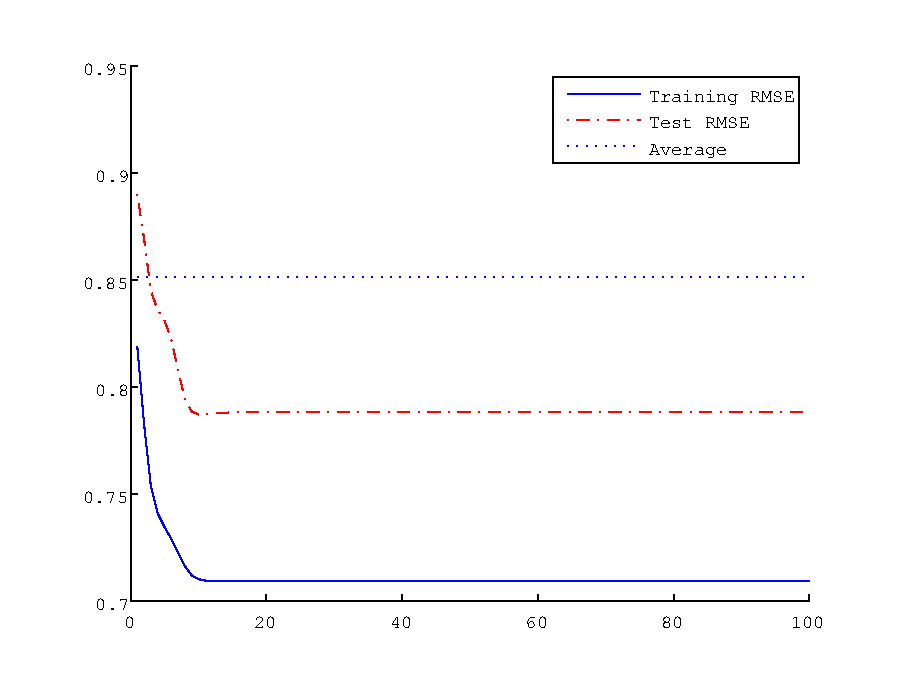
\includegraphics[scale=0.7]{figure/lrem_typical_plot}
  \end{center}
  \caption{Typical result when $d = 2$ and (Ratio of missing element)=0.5. The dotted line shows the RMSE when the estimation is simply the average rating of each movie (i.e. zero-order estimation)}
  \label{fig:lrem_typical_plot}
\end{figure}

Table \ref{table:lrem_result} compares the average RMSE of ten runs with the different dimensions of the low-rank approximation $d$ and the different ratio of the missing element in the rating matrix. Looking at the table in column-wise, it is found that the algorithm works better for the raining data with less missing ratings, which is an obvious result. An interesting result can be found by looking at the table in row-wise; larger dimension results in the larger RMSE when the rating matrix is sparse, but it results in the smaller RMSE when the rating matrix is mostly filled. It is because the algorithm badly overfits to the training data when the number of free parameters are large while the number of the available training data is small. 


\begin{table}[h]
 \caption{RMSE with different dimensions $d$ and different ratio of the missing element. The values are the average of ten runs.}
 \label{table:lrem_result}
 \begin{center}
  \begin{tabular}{|c|c||c|c|c|}
    \hline
    \multicolumn{2}{|c|}{}  & \multicolumn{3}{|c|}{Ratio of missing element in $R$} \\
    \cline{3-5}
     \multicolumn{2}{|c|}{}    &  0.7  &  0.5  & 0.2   \\
    \hline
    \hline
       & 1 &  0.808  &  0.795  &  0.789  \\
    \cline{2-5}
     $d$ & 2 &  0.859  &  0.790  & 0.772   \\
    \cline{2-5}
     & 3 &  0.933  &  0.808  &  0.772  \\
    \hline
  \end{tabular}
 \end{center}
\end{table}

\subsection{Complexity Analysis}
\paragraph{Time complexity} 
The most time consuming part of the algorithm is the $d$ by $d$ matrix inversion $(\check{M}^T\check{M})^{-1}$ in Eq. \ref{eq:lrem_core}. In practice, Gauss Elimination, which has a complexity of $\OO{n^3}$, is used to find the solution instead of complete matrix inversion. The inverse of matrix is computed $n_U+n_M$ times in each iteration. Thus the time complexity of the algorithm is 
\begin{equation}
\OO{d^3N(n_U+n_M)}
\end{equation}
where $N$ is the number of iterations.

\paragraph{Space complexity}
Only U and M are stored during computation. Thus the space complexity is
\begin{equation}
\OO{d(n_U+n_M)}.
\end{equation}

\subsection{Estimated performance on the full Netflix prize data}
\paragraph{Computational cost}
It took about 15 seconds for 100 iteration with $n_U=892$, $n_M=51$, and $d=3$ on Intel Celeron 2.0 GHz CPU. Thus for the full Netflix prize data where $n_U=480,189$ and $n_M=17,770$, the computation time for 100 iterations would take about 2 hours with $d=3$. Requied memory space would be about 11 MByte. Thus this is a tractable algorithm for the full Netflix prize data.

\paragraph{RMSE}
In the actual Netflix prize data 99.9\% elements of the rating matrix are missing. With the small data set where $n_U=892$, $n_M=51$, the algorithm cannot run with 99.9\% sparsity since $(\check{M}^T\check{M})^{-1}$ in Eq. \ref{eq:lrem_core} become singular for most of the rows due to the lack of data. One thing we can tell for sure from Table \ref{table:lrem_result} is that RMSE would be worse than 0.808 for the full Netflix prize data. Trying the algorithm on full data is the future work.



\if c\LaTeXe
\quad
\else
\end{document}
\fi




\if c\LaTeXe
\quad
\else

\documentclass{article}

\usepackage{amsmath, amssymb}
\usepackage{comment}
\usepackage{graphicx}
%\usepackage[T1]{fontenc}
%\usepackage{ae, aecompl}
\usepackage[numbers]{natbib}

%%%%%%%%%%%%%%%%%%%%%%%%%%%%%%%%%%%%%%%%%%%%%%%%%%%%%%%%%%%%%%%%%%%%%%%%
%% math

%
% General
%

\DeclareMathOperator{\argmin}{arg\,min}
\DeclareMathOperator{\argmax}{arg\,max}

%
% Sets
%

\newcommand{\card} [1]{{\lvert #1 \rvert}}
\newcommand{\range}[1]{{\left\{ 1, \dots, #1 \right\}}}

%
% Linear algebra
%

\newcommand{\mat}  [1]{{\bf #1}}
\newcommand{\norm} [1]{{\lVert #1 \rVert}}
\newcommand{\vect} [1]{{\mbox{\boldmath $#1$}}}

%
% Probability. The CTAN `proba` package doesn't seem to be that good.
% TODO ensuremath does not seem to be a good idea.
%

\newcommand{\E}    [2]{{\textrm{E} \left[ #1 \mid #2 \right]}}
\newcommand{\LL}   [2]{{\ensuremath{ L \left( #1 \,\middle|\, #2 \right) }}}
\newcommand{\LLL}  [2]{{\ensuremath{ l \left( #1 \,\middle|\, #2 \right) }}}
\newcommand{\N}    [1]{{\ensuremath{ \# \left( \textrm{ #1 } \right) }}}
\newcommand{\PO}   [1]{{\Pr \left( #1 \right)}}
\newcommand{\PP}   [2]{{\PO{ #1 \,\middle|\, #2 }}}

%%%%%%%%%%%%%%%%%%%%%%%%%%%%%%%%%%%%%%%%%%%%%%%%%%%%%%%%%%%%%%%%%%%%%%%%
%% Theoretical computer science

%
% Computational complexity
%

\DeclareMathOperator{\bigO}{O}
\providecommand{\OO}[1]{\bigO\bigl(#1\bigr)}

%%%%%%%%%%%%%%%%%%%%%%%%%%%%%%%%%%%%%%%%%%%%%%%%%%%%%%%%%%%%%%%%%%%%%%%%
%% General text

% \emph toggles italics; \textit sets italics; \em is deprecated
\newcommand{\term} [1]{{\emph{#1\/}}} 

% We don't need to do append a ~ or \ because TeX already handles .,
% correctly. TODO figure out if italics are correct here
\newcommand{\foreign}[1]{{\textit{#1}}}
\newcommand{\ea}      {{\foreign{et~al.}}}
\newcommand{\eg}      {{\foreign{e.g.}}}
\newcommand{\ie}      {{\foreign{i.e.}}}
\newcommand{\TODO} [1]{{\textbf{TODO}: \textit{#1}}}

%%%%%%%%%%%%%%%%%%%%%%%%%%%%%%%%%%%%%%%%%%%%%%%%%%%%%%%%%%%%%%%%%%%%%%%%
%% Remarks. Collected from the pervasive but untraceable `remarks.tex`.

\newif\ifremark
\long\def\remark#1{
\ifremark%
    \begingroup%
    \dimen0=\columnwidth
    \advance\dimen0 by -0.25in%
    \setbox0=\hbox{\parbox[b]{\dimen0}{\protect\em\textcolor{red}{#1}}}
    \dimen1=\ht0\advance\dimen1 by 2pt%
    \dimen2=\dp0\advance\dimen2 by 2pt%
    \vskip 0.25pt%
    \hbox to \columnwidth{%
        \vrule height\dimen1 width 3pt depth\dimen2%
        \hss\copy0\hss%
        \vrule height\dimen1 width 3pt depth\dimen2%
    }%
    \endgroup%
\fi}

\newcommand{\remarkname}[2] {
    \remark{{\bf #1}:#2}
}


\begin{document}

\fi

\section{Linear Regression + EM-like alternate update}
\subsection{Overview}
The goal of the algorithm is to find a low-rank approximation of the sparse rating matrix
\begin{equation}
R \approx MU
\end{equation}
where $M$ is a $n_M$-by-$d$ movie property matrix, $U$ is a
$d$-by-$n_U$ user property matrix, and $d$ is the dimension of the
low-rank approximation. Due to the missing entries of $R$, $M$ and $U$
cannot be obtained from singular value decomposition. Instead, the
algorithm learns $M$ and $U$ using linear regression and an EM-like
alternate update algorithm.

The time and space complexity of the algorithm is proportional to the data size $(n_U+n_M)$, so it is tractable even for the huge data set as in the Netflix prize. However, it poorly overfits to the training data especially when the rating matrix is sparse.

\subsection{Learning Algorithm}

At the beginning of the algorithm, $M$ is randomly initialized and fixed. Then the $i$th column of $U$ is learned by regular linear regression as follows;
\begin{equation}
\vect{u}_i=(\check{M}^T\check{M})^{-1}\check{M}^T \check{\vect r}_i \label{eq:lrem_core}
\end{equation}
Where $\check{\vect r}_i$ is a column vector constructed from the $i$th column of the rating matrix $R$, by excluding the missing elements from it. For example, if the $i$th column of $R$ is $[2 \quad \circ \quad 4 \quad \circ \quad \circ \quad 5 \quad \circ]^T$ where``$\circ$'' means missing element, then $\check{r}_i = [2 \quad 4 \quad 5]^T$. $U_i$ is a matrix with the corresponding columns of $U$.

Then $U$ is fixed in the next step, and each row of $M$ is updated in the exactly same manner. These steps are repeated until the training RMSE converges, just as EM algorithm. 

The important fact is that, by repeating this iteration, the training RMSE monotonically decreases, and eventually converges to the (local) optimum. Linear regression finds the parameter which minimizes the log likelihood given the following normal distribution with arbitrary fixed variance $\sigma^2$;
\begin{equation}
r_{i,j}\sim N(\vec{m}_i \cdot {\vect u}_j, \sigma^2)
\end{equation}
where $\vec{m}_i$ is the $i$ th row of $M$ and ${\vect u}_j$ is $j$ th column of $U$.

Thus, just as EM algorithm, the log likelihood on the training data monotonically decreases in each iteration. The RMSE is exactly same as the log likelihood when $\sigma = 1/\sqrt{2}$. Thus, the training RMSE monotonically decreases by iterations.

\subsection{Estimation}
Given the trained matrices $U$ and $M$, the maximum likelihood estimation of the ratings can be easily obtained as follows;
\begin{equation}
\hat{r}_{i,j}=\vec{m}_i \cdot {\vect u}_j
\end{equation}

Although the actual ratings are given as integer numbers from one to five, the estimations by this algorithm are real numbers. We use the real number outputs without rounding them. However, since ratings are from one to five, the estimations above five are turned into five, and those below one are turned into one. We call it \textit{rating range correction}\footnote{Is there more appropriate name for this....??}.

\subsection{Result}

Since the initial value of $M$ is randomly chosen, the result is stochastic. In fact it appears that the result is very sensitive to the initial value of $M$. Figure \ref{fig:lrem_typical_plot} shows the typical result of training RMSE and test RMSE as well as the RMSE when the estimation is simply the average rating of each movie (i.e. zero-order estimation). The training RMSE monotonically decreases over iterations as we expected, but test RMSE does not necessarily monotonically decreases. There is a large gap between training RMSE and test RMSE, indicating that the algorithm poorly overfits to the training data.

\begin{figure}[h]
  \begin{center}
    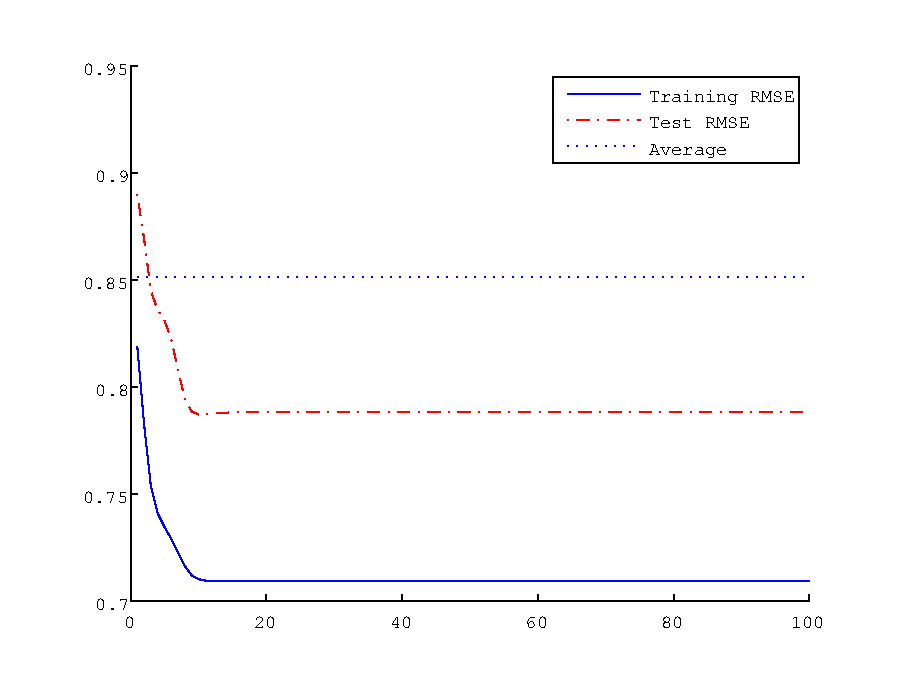
\includegraphics[scale=0.7]{figure/lrem_typical_plot}
  \end{center}
  \caption{Typical result when $d = 2$ and (Ratio of missing element)=0.5. The dotted line shows the RMSE when the estimation is simply the average rating of each movie (i.e. zero-order estimation)}
  \label{fig:lrem_typical_plot}
\end{figure}

Table \ref{table:lrem_result} compares the average RMSE of ten runs with the different dimensions of the low-rank approximation $d$ and the different ratio of the missing element in the rating matrix. Looking at the table in column-wise, it is found that the algorithm works better for the raining data with less missing ratings, which is an obvious result. An interesting result can be found by looking at the table in row-wise; larger dimension results in the larger RMSE when the rating matrix is sparse, but it results in the smaller RMSE when the rating matrix is mostly filled. It is because the algorithm badly overfits to the training data when the number of free parameters are large while the number of the available training data is small. 


\begin{table}[h]
 \caption{RMSE with different dimensions $d$ and different ratio of the missing element. The values are the average of ten runs.}
 \label{table:lrem_result}
 \begin{center}
  \begin{tabular}{|c|c||c|c|c|}
    \hline
    \multicolumn{2}{|c|}{}  & \multicolumn{3}{|c|}{Ratio of missing element in $R$} \\
    \cline{3-5}
     \multicolumn{2}{|c|}{}    &  0.7  &  0.5  & 0.2   \\
    \hline
    \hline
       & 1 &  0.808  &  0.795  &  0.789  \\
    \cline{2-5}
     $d$ & 2 &  0.859  &  0.790  & 0.772   \\
    \cline{2-5}
     & 3 &  0.933  &  0.808  &  0.772  \\
    \hline
  \end{tabular}
 \end{center}
\end{table}

\subsection{Complexity Analysis}
\paragraph{Time complexity} 
The most time consuming part of the algorithm is the $d$ by $d$ matrix inversion $(\check{M}^T\check{M})^{-1}$ in Eq. \ref{eq:lrem_core}. In practice, Gauss Elimination, which has a complexity of $\OO{n^3}$, is used to find the solution instead of complete matrix inversion. The inverse of matrix is computed $n_U+n_M$ times in each iteration. Thus the time complexity of the algorithm is 
\begin{equation}
\OO{d^3N(n_U+n_M)}
\end{equation}
where $N$ is the number of iterations.

\paragraph{Space complexity}
Only U and M are stored during computation. Thus the space complexity is
\begin{equation}
\OO{d(n_U+n_M)}.
\end{equation}

\subsection{Estimated performance on the full Netflix prize data}
\paragraph{Computational cost}
It took about 15 seconds for 100 iteration with $n_U=892$, $n_M=51$, and $d=3$ on Intel Celeron 2.0 GHz CPU. Thus for the full Netflix prize data where $n_U=480,189$ and $n_M=17,770$, the computation time for 100 iterations would take about 2 hours with $d=3$. Requied memory space would be about 11 MByte. Thus this is a tractable algorithm for the full Netflix prize data.

\paragraph{RMSE}
In the actual Netflix prize data 99.9\% elements of the rating matrix are missing. With the small data set where $n_U=892$, $n_M=51$, the algorithm cannot run with 99.9\% sparsity since $(\check{M}^T\check{M})^{-1}$ in Eq. \ref{eq:lrem_core} become singular for most of the rows due to the lack of data. One thing we can tell for sure from Table \ref{table:lrem_result} is that RMSE would be worse than 0.808 for the full Netflix prize data. Trying the algorithm on full data is the future work.



\if c\LaTeXe
\quad
\else
\end{document}
\fi






\section{Appendix}

\subsection{Mixture Models}

Here are the variables we're using for the mixture models:

\begin{itemize}
\item $\theta$: the entire set of parameters. TODO explain the sharing
  (but not here)
  \begin{itemize}
  \item $\theta^U_i(u)$: the probability distribution over user types
    $u$ for a user $i$ (think
    of this as a table). This is shared by all user-movie ratings for
    user $i$.
  \item $\theta^M_j(m)$: the probability distribution over movie
    types $m$ for a movie $j$. This is shared by all user-movie ratings for movie $j$.
  \item $\theta^R_{u,m}(r)$: the probability distributions over
    ratings $r$ for user type $u$ and movie type $m$. This is shared
    by all user-movie ratings $i,j$.
  \end{itemize}
\item Dimensions and sets
  \begin{itemize}
  \item $n_U$: number of users
  \item $n_M$: number of movies
  \item $k_U$: number of user types
  \item $k_M$: number of movie types
  \item $I$: the set of indexes $i,j$ of observed ratings
  \end{itemize}
\item Indexes. This allows us to omit ranges in sums and quantifiers.
  \begin{itemize}
  \item $i$: generally used to index over users
  \item $j$: generally used to index over movies
  \item $u$: generally used to index over user types
  \item $m$: generally used to index over movie types
  \end{itemize}
\item Random variables
  \begin{itemize}
  \item $U_i$: the user type of user $i$
  \item $M_j$: the movie type of movie $j$
  \item $R_{i,j}$: the rating user $i$ gave for movie $j$
  \end{itemize}
\end{itemize}

%% Bibliography
%\setlength{\bibsep}{2pt}
\footnotesize
\bibliography{refs}
\bibliographystyle{abbrvnat}

\end{document}

%%%%%%%%%%%%%%%%%%%%%%%%%%%%%%%%%%%%%%%%%%%%%%%%%%%%%%%%%%%%%%%%%%%%%%%%

\begin{comment}

\subsection{Mixture Model 1}

TODO insert graphical model

The likelihood of our model is:

\begin{align*}
  L \left( D \mid \theta \right)
  =& \PP{ R_{1,1} = r_{1,1}, \dots, R_{n,m} = r_{n,m} }{ \theta } \\
  =& \prod_{i,j} \PP{ R_{i,j} = r_{i,j} }{ \theta } \\
  =& \prod_{i,j} \sum_{u,m}
  \PP{ R_{i,j} = r_{i,j} }{ U_i = u, M_j = m, \theta_R }
  \PP{ U_i = u }{ \theta_U }
  \PP{ M_j = m }{ \theta_M } \\
  =& \prod_{i,j} \sum_{u,m} \theta_R(r \mid u,m) \theta_U(u) \theta_M(m)
\end{align*}

E-step:

\begin{align*}
  \forall i,j:
  & \PP{ U_i = u, M_j = m }{ R_{i,j} = r_{i,j}, \theta } \\
  =& \frac{
    \PP{ U_i = u, M_j = m, R_{i,j} = r_{i,j} }{ \theta }
  }{
    \PP{ R_{i,j} = r_{i,j} }{ \theta }
  } \\
% P(U,M|R) = P(U,M,R) = P(R|U,M) P(U,M)
  =& \frac{
    \PP{ U_i = u, M_j = m }{ \theta }
    \PP{ R_{i,j} = r_{i,j} }{ U_i = u, M_j = m, \theta }
  }{
    \sum_{u',m'}
    \PP{ U_i = u', M_j = m' }{ \theta }
    \PP{ R_{i,j} = r_{i,j} }{ U_i = u', M_j = m', \theta }
  } & \textrm{Bayes' rule} \\
  =& \frac{
    \PP{ U_i = u }{ \theta_U }
    \PP{ M_i = m }{ \theta_M }
    \PP{ R_{i,j} = r_{i,j} }{ U_i = u, M_j = m, \theta }
  }{
    \sum_{u',m'}
    \PP{ U_i = u' }{ \theta_U }
    \PP{ M_i = m' }{ \theta_M }
    \PP{ R_{i,j} = r_{i,j} }{ U_i = u', M_j = m', \theta }
  } & \textrm{Bayes' rule} \\
  =& \PP{}{}
\end{align*}

M-step:

\begin{align*}
\forall i,j: &
\PP{ R_{i,j} = r }{ U_i = u, M_j = m, \theta_R } \\
\forall i: &
\PP{ U_i = u }{ \theta_U } \\
=& \frac{
  \N{cells with user type $i$}
}{
  \N{cells}
}\\
=& \N{}
\end{align*}

TODO finish/correct above equations

\end{comment}
